\PassOptionsToPackage{dvipsnames}{xcolor}  % avoid options class with metropolis theme
\documentclass[aspectratio=169]{beamer} 

\usepackage{hayesmacros}

\usetheme[numbering=none, block=fill]{metropolis}
\setsansfont{Fira Sans}
\setmonofont{Fira Mono}

\usepackage{natbib}
\usepackage{nicematrix}
\usepackage{fontawesome5}

\newtheorem{proposition}{Proposition}
\newtheorem{assumption}{Assumption}
\theoremstyle{remark}
\newtheorem*{remark}{Remark}

\setbeamercolor{background canvas}{bg=white}
\setbeamercolor{normal text}{fg=black}
\setbeamercolor{frametitle}{bg=black, fg=white}

\hypersetup{colorlinks,allcolors=black}

\title{Minimax rates for the linear-in-means model reveal an identifiability-estimability gap}
\author{Alex Hayes}
\date{September 22, 2025 @ Stanford Metrics Lunch}

\institute{Joint work with Keith Levin at UW-Madison}

\begin{document}

\maketitle

\begin{frame}{My plan for today}
    
    \large
    
    1. Shameless introduction
    
    2. The linear-in-means model
    
    3. Dependence as a solution
    
    4. Why are folks parametric in 2025?
    
    5. Follow-up work (if time)
    
\end{frame}

\section{Shameless introduction}

\begin{frame}
    \vfill
    \begin{columns}
        \begin{column}{0.33\textwidth}
            \centering
            \includegraphics[height=0.35\textheight]{./figures/uw-crest-color-web-digital.pdf}
            
            PhD Student \\
            Statistics \\
            UW-Madison \\
            \vspace{4mm}
            Previously \\
            \vspace{6mm}
            \includegraphics[height=0.1\textheight]{./figures/RStudio.png} \hspace{0.5mm}
            \includegraphics[height=0.1\textheight]{./figures/Facebook_Logo_Primary.png} \hspace{0.5mm}
            \includegraphics[height=0.1\textheight]{./figures/broom.png}
        \end{column}
        \begin{column}{0.33\textwidth}
            \centering
            \includegraphics[height=0.35\textheight]{./figures/Block_S_3_color.png}
            
            Postdoc \\
            Economics \\
            Stanford \\
            \vspace{4mm}
            Now \\
            \vspace{6mm}
            \phantom{
                \includegraphics[height=0.1\textheight]{./figures/RStudio.png}
                \includegraphics[height=0.1\textheight]{./figures/Facebook_Logo_Primary.png}
            }
        \end{column}
        \begin{column}{0.33\textwidth}
            \centering
            \includegraphics[height=0.35\textheight]{./figures/oregon-state.png}
            
            Assistant Professor \\
            Statistics \\
            Oregon State \\
            \vspace{4mm}
            Next \\
            \vspace{6mm}
            \phantom{
                \includegraphics[height=0.1\textheight]{./figures/RStudio.png}
                \includegraphics[height=0.1\textheight]{./figures/Facebook_Logo_Primary.png}
            }
        \end{column}
    \end{columns}
    
\end{frame}

\begin{frame}{I'm working with Arun Chandrasekhar on methods for network experiments}
    \begin{columns}
        \begin{column}{0.5\textwidth}
            \textbf{Research interests:}
            \begin{itemize}
                \item (Social) networks
                \item Causal inference in noisy networks
                \item Semi-parametric mediation
                \item Social processes in science
                \item Software design, \texttt{\#rstats}
            \end{itemize}
        \end{column}
        \begin{column}{0.5\textwidth}
            In Landau 252, stop by anytime \\    
            \vspace{3mm}
            Happy to answer stats question
        \end{column}
    \end{columns}
\end{frame}

\section{The linear-in-means model}

\begin{frame}{Understanding social influence is fundamental in a highly connected society}
    
    \begin{columns}
        \begin{column}{0.35\textwidth}
            \centering
            \begin{tikzpicture}[scale=0.6]
                \node[shape=circle,fill=Mahogany] (A) at (0,1) {};
                \node[shape=circle,fill=gray,label=below left:{\includegraphics[scale=0.2]{./figures/bacteria.png}}] (B) at (1,-1) {};
                \node[shape=circle,fill=Mahogany] (C) at (1.5,2.5) {};
                \node[shape=circle,fill=Mahogany] (D) at (2.75,0.5) {};
                \node[shape=circle,fill=gray,label=above right:{\includegraphics[scale=0.2]{./figures/bacteria.png}}] (E) at (4.3,2.4) {};
                \node[shape=circle,fill=Mahogany,label=below:{\includegraphics[scale=0.2]{./figures/bacteria.png}}] (F) at (3.4,-1.4) {};
                \node[shape=circle,fill=gray,label=right:{\includegraphics[scale=0.2]{./figures/bacteria.png}}] (G) at (4.7,0.1) {};
                
                \draw (A) -- (B);
                \draw (A) -- (C);
                \draw (B) -- (C);
                \draw (B) -- (D) -- (F);
                \draw (C) -- (D) -- (E);
                \draw (B) -- (F) -- (G) -- (E) -- (C);
            \end{tikzpicture}
        \end{column}
        \begin{column}{0.65\textwidth}
            \vspace{6mm} \\
            \onslide<1->{
                \textbf{Direct effect}: if I get \textcolor{Mahogany}{vaccinated}, I am less likely to get sick \includegraphics[scale=0.2]{./figures/bacteria.png}
                \vspace{4mm} \\
                \textbf{Contagion}: if my friends get sick \includegraphics[scale=0.2]{./figures/bacteria.png}, I am more likely to get sick \includegraphics[scale=0.2]{./figures/bacteria.png}
                \vspace{4mm} \\
                \textbf{Interference}: if my friends get \textcolor{Mahogany}{vaccinated}, I am less likely to get sick \includegraphics[scale=0.2]{./figures/bacteria.png}
                \vspace{7mm} \\
            }
            \onslide<2->{
                \footnotesize * Can be defined counterfactually \citep{vazquez-bare2023}, but we do not consider counterfactual inference in this talk.
            }
        \end{column}
    \end{columns}
\end{frame}

\begin{frame}{Linear-in-means model are popular models for understanding social influence}
    Used widely in education, crime, health, social policy, etc \footnote{\cite{sacerdote2001, epple2011, soetevent2007, trogdon2008, duflo2003, bertrand2000, glaeser1996, patacchini2012a, carrell2013}, etc} \\
    \vspace{6mm}
    I'm interested in understanding this model but I don't necessarily endorse it
\end{frame}

\begin{frame}{Linear-in-means models are a canonical tool to estimate social influence}
    \footnotesize
    \begin{table}[]
        \begin{tabular}{llcl@{\hspace{4em}}lcl}
            \onslide<1->{Outcome         & (sick?)       & $Y_i$    & $\in \{0, 1\}$             & Base rate                  & $\alpha$ & $\in \R$}      \\
            \onslide<2->{Node degree     & (num friends) & $d_i$    & $\in \set{0, 1, 2, \dots}$ & Contagion                  & $\beta$  & $\in (-1, 1)$} \\
            \onslide<2->{Edge $i \sim j$ & (friends?)    & $A_{ij}$ & $\in \{0, 1\}$}            & \onslide<3->{Direct effect & $\gamma$ & $\in \R$ }     \\
            \onslide<3->{Treatment       & (vaccinated?) & $T_i$    & $\in \{0, 1\}$ }           & \onslide<4->{Interference  & $\delta$ & $\in \R$}      \\
        \end{tabular}
    \end{table}
    \Large
    \vspace{4mm}
    \begin{equation*}
        \onslide<1->{
            \underbrace{Y_i}_\text{sick?} =
            \alpha
        }
        \onslide<2->{
            + \beta \underbrace{\frac{1}{d_i} \sum_{j \, : \, A_{ij} = 1} Y_j}_{\substack{\text{fraction} \\ \text{sick} \\ \text{friends}}}
        }
        \onslide<3->{
            + \gamma \underbrace{T_i}_\text{vaccinated?}
        }
        \onslide<4->{
            + \delta \underbrace{\frac{1}{d_i} \sum_{j \, : \, A_{ij} = 1} T_j}_{\substack{\text{fraction} \\ \text{vaccinated} \\ \text{friends}}}
        }
        \onslide<5-> {
            + \underbrace{\varepsilon_i}_\text{error}
        }
    \end{equation*}
    
    \onslide<6->{\footnotesize Letting $G = D^{-1} A$ be the row-normalized adjacency matrix, can write in matrix-vector form: \Large
        \begin{equation*} \label{eq:lim-mv}
            Y = \alpha 1_n + \beta G Y + T \gamma + G T \delta + \varepsilon
        \end{equation*}
    }
\end{frame}

\begin{frame}{Linear-in-means models are closely connected to spatial autoregression models}
    \centering
    \includegraphics[height=0.95\textheight]{./figures/oregon_map.png}
\end{frame}

\begin{frame}{Identification in the linear-in-means model can be subtle}
    \centering
    \includegraphics[height=0.95\textheight, page=2, trim={0 14cm 0 0}, clip]{./papers/manski.pdf}
\end{frame}


\begin{frame}{Linear-in-means models are famously suspectible to perfect collinearity}
    \begin{minipage}{0.49\textwidth}
        \centering
        \begin{tikzpicture}
            \node[shape=circle,fill=Mahogany,label=above left:{$T_1 = 1$}] (A) at (0,1) {};
            \node[shape=circle,fill=gray,label=below left:{$T_2 = 0$}] (B) at (1,0) {};
            \node[shape=circle,fill=Mahogany,label=above right:{$T_3 = 1$}] (C) at (1.5,1.5) {};
            \node[shape=circle,fill=Mahogany,label=above right:{$T_4 = 1$}] (D) at (2.75,0.5) {};
            
            \path (A) edge [loop above] node {} (A);
            \path (B) edge [loop below] node {} (B);
            \path (C) edge [loop above] node {} (C);
            \path (D) edge [loop above] node {} (D);
            
            \draw (A) -- (B);
            \draw (A) -- (C);
            \draw (A) -- (D);
            \draw (B) -- (C);
            \draw (B) -- (D);
            \draw (C) -- (D);
        \end{tikzpicture}
    \end{minipage}
    \begin{minipage}{0.49\textwidth}
        \centering
        \begin{tikzpicture}
            \node[shape=circle,fill=Mahogany,label=above left:{$[GT]_1 = 3/4$}] (A) at (0,1) {};
            \node[shape=circle,fill=gray,label=below left:{$[GT]_2 = 3/4$}] (B) at (1,0) {};
            \node[shape=circle,fill=Mahogany,label=above right:{$[GT]_3 = 3/4$}] (C) at (1.5,1.5) {};
            \node[shape=circle,fill=Mahogany,label=above right:{$[GT]_4 = 3/4$}] (D) at (2.75,0.5) {};
            
            \path (A) edge [loop above] node {} (A);
            \path (B) edge [loop below] node {} (B);
            \path (C) edge [loop above] node {} (C);
            \path (D) edge [loop above] node {} (D);
            
            \draw (A) -- (B);
            \draw (A) -- (C);
            \draw (A) -- (D);
            \draw (B) -- (C);
            \draw (B) -- (D);
            \draw (C) -- (D);
        \end{tikzpicture}
    \end{minipage}
    
    \begin{equation*}
        \begin{bmatrix}
            Y_1 \\
            Y_2 \\
            Y_3 \\
            Y_4
        \end{bmatrix}
        =
        \begin{bNiceMatrix}[first-row,first-col]
             & 1_n                     & GY   & T & GT                        \\
             & \textcolor{Mahogany}{1} & GY_1 & 1 & \textcolor{Mahogany}{3/4} \\
             & \textcolor{Mahogany}{1} & GY_2 & 0 & \textcolor{Mahogany}{3/4} \\
             & \textcolor{Mahogany}{1} & GY_3 & 1 & \textcolor{Mahogany}{3/4} \\
             & \textcolor{Mahogany}{1} & GY_4 & 1 & \textcolor{Mahogany}{3/4} \\
        \end{bNiceMatrix}
        \begin{bmatrix}
            \textcolor{Mahogany}{\alpha} \\
            \beta                        \\
            \gamma                       \\
            \textcolor{Mahogany}{\delta}
        \end{bmatrix}
        +
        \begin{bmatrix}
            \varepsilon_1 \\
            \varepsilon_2 \\
            \varepsilon_3 \\
            \varepsilon_4
        \end{bmatrix}
    \end{equation*}
    
    \centering
    Can't distinguish base rate $\textcolor{Mahogany}{\alpha}$ from interference $\textcolor{Mahogany}{\delta}$ due to collinearity
\end{frame}

\begin{frame}{It's widely believed that this ``reflection problem'' is rarely a problem in practice}
    
    \begin{proposition}[\citealt{bramoulle2009}]
        Suppose $\gamma \beta + \delta \neq 0$. If $I, G$ and $G^2$ are linearly independent, i.e., that $a I + b G + c G^2 = 0$ requires $a = b = c = 0$, then $\alpha, \beta, \gamma$ and $\delta$ are identified.
    \end{proposition}
    
    There is no perfect collinearity and peer influence is identified when there are \textcolor{Mahogany}{open triangles} (``intransitivity'') in the network
    \begin{columns}
        \begin{column}{0.5\textwidth}
            \centering
            \begin{tikzpicture}
                \node[shape=circle,fill=gray,label=above left:A] (A) at (0,1) {};
                \node[shape=circle,fill=Mahogany,label=below left:B] (B) at (1,0) {};
                \node[shape=circle,fill=Mahogany,label=above right:C] (C) at (1.5,1.5) {};
                \node[shape=circle,fill=Mahogany,label=above right:D] (D) at (2.75,0.5) {};
                \draw (A) -- (B);
                \draw (A) -- (C);
                \draw (B) -- (C);
                \draw (C) -- (D);
            \end{tikzpicture}
        \end{column}
        \begin{column}{0.5\textwidth}
            \centering
            Open: \textcolor{Mahogany}{$B \leftrightarrow C \leftrightarrow D \nleftrightarrow B$} \\
            Closed: $A \leftrightarrow B \leftrightarrow C \leftrightarrow A$
        \end{column}
    \end{columns}
    \vspace{2mm}
    \textbf{Standard wisdom} is that collinearity is \textbf{not a problem} because most networks have open triangles
\end{frame}

% \begin{frame}{It's widely believed that this ``reflection problem'' is rarely a problem in practice}
%     \begin{proposition}[\citealt{bramoulle2009}]
%         Suppose there are no isolated nodes in the network. Then $(\alpha, \beta, \gamma, \delta)$ are identified if and only if $1_n, \E[T, GT]{GY}, T$ and $GT$ are linearly independent.
%     \end{proposition}
%     \begin{equation*}
%         \begin{bmatrix}
%             Y_1    \\
%             Y_2    \\
%             \vdots \\
%             Y_n
%         \end{bmatrix}
%         =
%         \begin{bmatrix}
%             1      & [GY]_1 & T_1    & [GT]_1 \\
%             1      & [GY]_2 & T_2    & [GT]_2 \\
%             \vdots & \vdots & \vdots & \vdots \\
%             1      & [GY]_n & T_n    & [GT]_n \\
%         \end{bmatrix}
%         \begin{bmatrix}
%             \alpha \\
%             \beta  \\
%             \gamma \\
%             \delta
%         \end{bmatrix}
%         +
%         \begin{bmatrix}
%             \varepsilon_1 \\
%             \varepsilon_2 \\
%             \vdots        \\
%             \varepsilon_n
%         \end{bmatrix}
%     \end{equation*} \\
%     \vspace{4mm}
%     Very similar to the usual requirement in linear models that the columns of the design matrix are linearly independent
% \end{frame}

\begin{frame}{We came up with a new estimator for the linear-in-means model}
    
    \textbf{Setting}: Treatment random and independent of network. $T_i \diid \Bern(0.5)$ \\
    
    \Large
    \begin{equation*}
        Y = \alpha 1_n + \beta G Y + T \gamma + G T \delta + \varepsilon
    \end{equation*}
    
    \normalsize
    We started to run a simulation study\footnote{Generate $Y$ via the reduced-form specification $Y = \paren*{I - \beta G}^{-1} \paren*{\alpha 1_n + \gamma T + \delta G T + \varepsilon}$} to confirm that our estimator worked...
    
\end{frame}

\begin{frame}{In our simulations, the network had many open triangles...}
    \centering
    \includegraphics{./figures/simulations/jobtalk-backbone.pdf}
\end{frame}

\begin{frame}{...but we couldn't estimate peer effects!}
    It wasn't just us, none of the standard estimators worked!
    \begin{figure}
        \centering
        \includegraphics[width=\textwidth]{./figures/simulations/jobtalk-mse.pdf}
    \end{figure}
\end{frame}

\begin{frame}{The issue: the interference column converges to a constant in large samples}
    \centering
    \onslide<3->{
        When the network grows ($n \to \infty$),
    }
    \onslide<4->{
        if everyone makes more friends ($d_i \to \infty$)
    }
    \Large
    \vspace{6mm}
    \begin{equation*}
        \onslide<3->{
            \lim_{n \to \infty}
        }
        \onslide<1->{
            \underbrace{[GT]_i}_{\substack{\text{fraction} \\ \text{vaccinated} \\ \text{friends}}}
        }
        \onslide<2->{=}
        \onslide<3->{
            \lim_{n \to \infty}
        }
        \onslide<2->{
            \underbrace{
                \frac{1}{d_i} \sum_{j \, : \, A_{ij} = 1} T_j
            }_{\substack{\text{average of $d_i$}           \\ \text{i.i.d. coin flips}}}
        }
        \onslide<4->{
            = \frac 12   
        }
    \end{equation*} \\
    \normalsize
    \vspace{6mm}
    \onslide<5->{
        \underline{For every single node $i = 1, ..., n$}
    }
\end{frame}

\begin{frame}{Base rates and interence are collinear in large samples}
    \centering
    \begin{equation*}
        \begin{bmatrix}
            Y_1    \\
            Y_2    \\
            \vdots \\
            Y_n
        \end{bmatrix}
        =
        \underbrace{
            \begin{bNiceMatrix}[first-row,first-col]
                 & 1_n                     & GY     & T      & GT                        \\
                 & \textcolor{BrickRed}{1} & GY_1   & 1      & \textcolor{BrickRed}{1/2} \\
                 & \textcolor{BrickRed}{1} & GY_2   & 0      & \textcolor{BrickRed}{1/2} \\
                 & \vdots                  & \vdots & \vdots & \vdots                    \\
                 & \textcolor{BrickRed}{1} & GY_n   & 1      & \textcolor{BrickRed}{1/2}
            \end{bNiceMatrix}
        }_\text{as $n \to \infty$}
        \begin{bmatrix}
            \textcolor{BrickRed}{\alpha} \\
            \beta                        \\
            \gamma                       \\
            \textcolor{BrickRed}{\delta}
        \end{bmatrix}
        +
        \begin{bmatrix}
            \varepsilon_1 \\
            \varepsilon_2 \\
            \vdots        \\
            \varepsilon_n
        \end{bmatrix}
    \end{equation*} \\
    \vspace{8mm}
    \underline{Sometimes can't distinguish between base rate $\textcolor{BrickRed}{\alpha}$ and interference $\textcolor{BrickRed}{\delta}$}
\end{frame}

\begin{frame}{In simulations, we couldn't estimate $\textcolor{BrickRed}{\beta}$ either}
    \begin{figure}
        \centering
        \includegraphics[width=\textwidth]{./figures/simulations/jobtalk-mse.pdf}
    \end{figure}
\end{frame}

\begin{frame}{Outcomes are generated by diffusing the treatment over the network}
    Why is $\textcolor{BrickRed}{\beta}$ also affected?
    \begin{align*}
        \onslide<1-> {
        Y             & = \alpha 1_n + \beta G Y + \gamma T + \delta G T + \varepsilon                        \\
        }
        \onslide<2-> {
        Y - \beta G Y & = \alpha 1_n  + \gamma T + \delta G T + \varepsilon                                   \\
        }
        \onslide<3->{
        Y             & = \paren*{I - \beta G}^{-1} \paren*{\alpha 1_n + \gamma T + \delta G T + \varepsilon} \\
        }
        \onslide<4->{
                      & \overset{*}{=} \underbrace{\sum_{k=0}^\infty \beta^k G^k}_{\substack{\text{repeated}  \\ \text{neighborhood} \\ \text{averaging}}} \paren*{\alpha 1_n + \gamma T + \delta G T + \varepsilon} \\
        }
    \end{align*}
    \footnotesize
    \onslide<4->{* Must have $\abs{\beta} < 1$, so effect of averaging decays with repetition}
\end{frame}

\begin{frame}{The contagion column converges to a constant in large samples}
    \begin{align*}
        GY = 
        \frac{\alpha}{1 - \beta} 1_n + 
        \underbrace{\gamma G T}_{\substack{\text{neighborhood}                                              \\ \text{average } \to \gamma / 2}} + 
        \underbrace{(\gamma \beta + \delta) \sum_{k=0}^\infty \beta^k G^{k+2} T}_{\substack{\text{repeated} \\ \text{neighborhood} \\ \text{averages} \\ \text{of $T$ *}}} +
        \underbrace{\sum_{k=0}^\infty \beta^k G^{k+1} \varepsilon}_{\substack{\text{repeated}               \\ \text{neighborhood} \\ \text{averages} \\ \text{of $\varepsilon$ } \to \, 0}}
    \end{align*} \\
    \vspace{4mm}
    Each term in the sum converges to a constant
    \begin{align*}
        GY & \to \eta
    \end{align*} \\
    \vspace{4mm}
    \footnotesize
    * Neighborhood average of a constant is that same constant
\end{frame}

\begin{frame}{Base rates, interference and contagion are collinear in large samples}
    
    \begin{equation*}
        \begin{bmatrix}
            Y_1    \\
            Y_2    \\
            \vdots \\
            Y_n
        \end{bmatrix}
        =
        \underbrace{
            \begin{bNiceMatrix}[first-row,first-col]
                 & 1_n                     & GY                         & T      & GT                        \\
                 & \textcolor{BrickRed}{1} & \textcolor{BrickRed}{\eta} & 1      & \textcolor{BrickRed}{1/2} \\
                 & \textcolor{BrickRed}{1} & \textcolor{BrickRed}{\eta} & 0      & \textcolor{BrickRed}{1/2} \\
                 & \vdots                  & \vdots                     & \vdots & \vdots                    \\
                 & \textcolor{BrickRed}{1} & \textcolor{BrickRed}{\eta} & 1      & \textcolor{BrickRed}{1/2}
            \end{bNiceMatrix}
        }_\text{as $n \to \infty$}
        \begin{bmatrix}
            \textcolor{BrickRed}{\alpha} \\
            \textcolor{BrickRed}{\beta}  \\
            \gamma                       \\
            \textcolor{BrickRed}{\delta}
        \end{bmatrix}
        +
        \begin{bmatrix}
            \varepsilon_1 \\
            \varepsilon_2 \\
            \vdots        \\
            \varepsilon_n
        \end{bmatrix}
    \end{equation*} \\
    \vspace{6mm}
    \begin{center}
        \underline{Sometimes can't distinguish between base rate $\textcolor{BrickRed}{\alpha}$, interference $\textcolor{BrickRed}{\delta}$ and contagion $\textcolor{BrickRed}{\beta}$} \\
    \end{center}
\end{frame}

\begin{frame}{Peer effects are asymptotically collinear under random experiments}
    \begin{assumption}
        \begin{enumerate}
            \item $T_1,T_2,\dots,T_n$ are independent with shared mean $\tau \in \R$, and $T$ is independent of $A$.
            \item $\{ T_i - \tau : i \in [n] \}$ are independent subgamma$^*$ random variables.
            \item $\varepsilon_1, \varepsilon_2, \dots, \varepsilon_n$ are independent subgamma random variables.
            \item The minimum degree grows strictly faster than $\log n$, such that
                  \begin{equation*}
                      \lim_{n \to \infty} \frac{\min_{i \in [n]} d_i}{\log n} = \infty.
                  \end{equation*}
        \end{enumerate}
    \end{assumption}
    
    $^*$\underline{Examples}: Bernoulli, Poisson, Exponential, Gamma, Gaussian, sub-Gaussian, squared sub-Gaussians, bounded distributions, etc
\end{frame}

\begin{frame}{The interference and contagion columns converge uniformly to constants}
    
    \begin{theorem}
        Under the previous assumptions,
        \begin{equation*}
            \max_{i \in [n]} \Big| [GT]_i - \tau \Big|
            = o(1) ~ \text{ almost surely }
        \end{equation*}
        and there exists $\eta \in \R$ such that
        \begin{equation*}
            \max_{i \in [n]} \Big| [GY]_i - \eta \Big|
            = o(1) ~ \text{ almost surely.}
        \end{equation*}
    \end{theorem}
\end{frame}

\begin{frame}{This result covers weighted and directed networks}
    \textbf{Weighted networks}: If $A \in \R^{n \times n}_{\ge 0}$ is a positive, weighted network with $(\nu, b)$-subgamma edges $A_{ij}$, we require that
    \begin{equation*}
        \max_{i \in [n]} \frac{1}{d_i^2} \sum_{j=1}^n A_{ij}^2
        = o\left( \frac{ 1 }{ \nu \log^2 n } \right)
        ~\text{ and }~
        \max_{j \in [n]} \frac{ A_{ij} }{ d_i }
        = o\left( \frac{ 1 }{ b \log n } \right).
    \end{equation*} \\
    Roughly: no one edge can be too important for a given node \\
    \vspace{4mm}
    \textbf{Directed networks}: extension possible, but slightly more involved
\end{frame}

\begin{frame}{Collinearity shows up quickly in finite samples}
    \vspace{3mm}
    \centering
    \includegraphics{./figures/simulations/defense-vif.pdf}
\end{frame}

\begin{frame}{Minimax lower bounds show asymptotic collinearity can lead to inconsistency}
    
    \begin{theorem}[Hayes and Levin 2025]
        Let $\Theta_\mathrm{LIM}= \left\{ (\alpha,\beta,\gamma,\delta) : \alpha,\gamma,\delta \in \R, \beta \in (-1,1) \right\}$ and suppose that $\varepsilon \sim \mathcal N(0, \sigma^2 I)$. There exist positive constants $c_\beta,c_\delta$ and $c_0$, such that for sufficiently large $n$
        \begin{equation*} \label{eq:minimax:betadelta}
            \inf_{\widehat{\theta}} \sup_{\theta \in \Theta_\mathrm{LIM}}
            \min\left\{
            \mathbb{P}_{\theta}\left[
                \left| \betahat - \beta \right| \ge \frac{c_\beta}{\| G \|_F} \right] ,
            ~
            \mathbb{P}_{\theta}\left[
                \left| \deltahat - \delta \right| \ge \frac{c_\delta}{\| G \|_F} \right]
            \right\} 
            \ge c_0 ,
        \end{equation*}
        where the infimum is over all estimators. Further, if $\tau \neq 0$, there exist positive constants $c_\alpha$ and $c_\alpha'$ such that
        \begin{equation*}
            \inf_{\widehat{\theta}} \sup_{\theta \in \Theta_\mathrm{LIM}}
            \mathbb{P}_{\theta}\left[
                \left| \alphahat - \alpha \right| \ge \frac{c_\alpha}{\| G \|_F} \right]
            \ge c_\alpha' .
        \end{equation*}
    \end{theorem}
\end{frame}


\begin{frame}{Minimax lower bounds show asymptotic collinearity can lead to inconsistency}
    
    In binary networks, $\| G \|_F = \sqrt{n/\bar{d}_{\text{har}}}$, where $\displaystyle \bar{d}_{\text{har}} = \frac{n}{\sum_{i=1}^n 1/d_i}$.
    
    \vspace{3mm}
    
    Since the harmonic mean is lower bounded by the minimum, we have:
    
    \vspace{2mm}
    
    \begin{theorem}[Intuitive]
        In the worst case scenarios, $\alpha, \beta$ and $\delta$ cannot be estimated faster than $\sqrt{n / d_{\min}}$, where $d_{\min} = \min_{i \in [n]} d_i$.
    \end{theorem}
    
    \vspace{2mm}
    
    If $d_{\min}$ diverges, we cannot obtain parametric rates and if $d_{\min} = \Omega(n)$, consistent estimation is impossible over $\Theta_\mathrm{LIM}$.$^*$ \\
    \vspace{4mm}
    \footnotesize$^*$ A vanishing fraction of nodes may have bounded degree, since bound is actually in $\bar{d}_{\text{har}}$
    
\end{frame}



\begin{frame}{The standard wisdom about linear-in-means model is incomplete}
    
    \textbf{Standard wisdom} states that collinearity isn't a problem in linear-in-means in networks with open triangles \citep{bramoulle2009} \\
    
    \vspace{4mm}
    But: \underline{identification does not justify inference}! Doesn't guarantee consistency! \\
    
\end{frame}

% \begin{frame}


%     \vspace{4mm}

%     \begin{block}{Takeaway 1}
%         When nodal covariates are independent of the network, we show that peer effects may not be estimable, due to collinearity, even when there are many open triangles.
%     \end{block}

%     \vspace{4mm}

%     \begin{block}{Takeaway 2}
%         Direct effects are estimable even when there is asymptotic collinearity.
%     \end{block}
% \end{frame}

\begin{frame}{Why hasn't the spatial econometrics literature encountered this issue before?}
    Theory directly assumes there is no asymptotic collinearity \\
    \vspace{3mm}
    Simulations rarely investigate consistency of estimators \\
    \vspace{3mm}
    Often treat covariates $T$ and network $G$ as fixed rather than random \\
    \vspace{6mm}
    \footnotesize *Recent work has explicitly leveraged asymptotic collinearity in random graphs to estimate direct effects \citep{li2022f}
\end{frame}

\begin{frame}{The network designs literature is well-aware of issues with Bernoulli designs}
    \vfill
    \centering
    \includegraphics[height=0.9\textheight, page=1, trim={1.5cm 4cm 2cm 5cm}, clip]{./papers/airoldi.pdf}
\end{frame}

\begin{frame}{The network designs literature is well-aware of issues with Bernoulli designs}
    \vfill
    \centering
    \includegraphics[height=0.9\textheight, page=1, trim={1.5cm 8.5cm 0 2cm}, clip]{./papers/gcr.pdf}
\end{frame}

\begin{frame}{The network designs literature is well-aware of issues with Bernoulli designs}
    \vfill
    \centering
    \includegraphics[height=0.95\textheight, page=1, trim={2.5cm 8cm 0 3cm}, clip]{./papers/conflict.pdf}
\end{frame}

\begin{frame}{The network designs literature is well-aware of issues with Bernoulli designs}
    \vfill
    \centering
    \includegraphics[height=0.95\textheight, page=1, trim={1.5cm 9cm 0 3.5cm}, clip]{./papers/viviano-clustering.pdf}
\end{frame}

\section{Dependence as a solution}

\begin{frame}{Dependence between treatment and network might resolve collinearity issues}
    \Large
    \begin{align*}
        \underbrace{[GT]_i}_{\substack{\text{fraction} \\ \text{vaccinated} \\ \text{friends}}}
        = \underbrace{
            \frac{1}{d_i} \sum_{j \, : \, A_{ij} = 1} T_j
        }_{\substack{\text{average of dependent treatments}}}
    \end{align*} \\
    \normalsize
    \centering
    \vspace{8mm}
    $GT$ might not converge, or might converge to non-constant value
\end{frame}

\begin{frame}{We considered models where treatment depended on position in network}
    \centering
    \includegraphics{./figures/simulations/defense-backbone-dependent.pdf}
\end{frame}

\begin{frame}{We considered models where treatment depended on position in network}
    
    \begin{columns}
        \column{0.45\textwidth}
        \centering
        \includegraphics[width=\textwidth]{./figures/assortative.png}
        \column{0.55\textwidth}
        
        Stochastic blockmodels are an intuitive way to induce dependence \\
        \vspace{4mm}
        
        Block indicators $Z_i$ \\
        Popularity parameters $\theta_i$ \\
        Mixing matrix $B \in [0, 1]^{d \times d}$
        
        \begin{equation*}
            \P[\Z, \theta]{A_{ij} = 1} = \theta_i Z_i B Z_j^T \theta_j
        \end{equation*}
    \end{columns}
\end{frame}

\begin{frame}{We prove a partial asymptotic collinearity result for these models}
    \begin{theorem}[Hayes and Levin 2025]
        Suppose that $A$ is sampled from a degree-corrected stochastic blockmodel. Define $X_i = \theta_i Z_i$. Let 
        \begin{equation*}
            Y = \alpha 1_n + \beta G Y + X \gamma + G X \delta + \varepsilon
        \end{equation*}
        for $\alpha, \beta \in \R$ and $\gamma, \delta \in \R^d$. Suppose that $X$ has $k \ge 2d$ distinct rows. Then, under suitable conditions,
        \begin{equation*}
            W_n = \begin{bmatrix}
                1_n & GY & X & GX
            \end{bmatrix}
        \end{equation*}
        converges uniformly to a limit object with rank $2d$ out of $2d + 2$. If two entries of $(\alpha, \beta, \delta_1, ..., \delta_d)$ are set to zero in the data generating process, the limit object of $W_n$ is a matrix with full rank.
    \end{theorem}
\end{frame}

\begin{frame}{We prove a partial asymptotic collinearity result for these models}
    \textbf{Key condition to avoid collinearity}: sufficient degree heterogeneity such that $X$ and $D^{-1} X$ are linearly independent
    
    \vspace{4mm}
    \textbf{General low-rank networks}: if $\bbE[ A_{ij} \mid X ] = X_i^T X_j$, a similar result holds, broadly generalizing the partial identification result
\end{frame}

\begin{frame}{We performed a simulation study to confirm the theoretical results}
    \begin{itemize}
        \setlength\itemsep{1.75em}
        \item \textcolor{BrickRed}{Bernoulli}: Treatment random and independent of network. $T_i \diid \Bern(0.5)$
              \begin{equation*}
                  Y = \textcolor{BrickRed}{\alpha} 1_n + \textcolor{BrickRed}{\beta} G Y + T \gamma + G T \textcolor{BrickRed}{\delta} + \varepsilon,
              \end{equation*}
              with $\textcolor{BrickRed}{\alpha} = 3, \textcolor{BrickRed}{\beta} = 0.2, \gamma = 4, \textcolor{BrickRed}{\delta} = 2$ and $\varepsilon \diid \calN(0, \sigma^2)$ with $\sigma = 0.1$.
        \item \textcolor{BrickRed}{Unrestricted model}: Treatment random and dependent on network. Define $X_i = \theta_i Z_i \in \R^4$
              \begin{equation*}
                  Y = \textcolor{BrickRed}{\alpha} 1_n + \textcolor{BrickRed}{\beta} G Y + X \gamma + G X \textcolor{BrickRed}{\delta} + \varepsilon,
              \end{equation*}
              where $\textcolor{BrickRed}{\alpha} = 3, \textcolor{BrickRed}{\beta} = 0.2$ and $\varepsilon \diid \calN(0, \sigma^2)$ with $\sigma = 0.1$. Since $X_i \in \R^4$, $\gamma, \textcolor{BrickRed}{\delta} \in \R^4$ and we fix $\textcolor{BrickRed}{\delta} = (2, 2, 2, 2)$ and $\gamma = (1.5, 2.5, 3.5, 4.5)$.
        \item Restricted model: The unrestricted model, but $\delta = (0, 0, 2, 2)$, so there's no asymptotic collinearity.
    \end{itemize}
\end{frame}

\begin{frame}{Dependence prevented \textcolor{BrickRed}{asymptotic collinearity} and estimation challenges}
    \centering
    \includegraphics[width=0.85\textwidth]{./figures/simulations/jobtalk-mse-all.pdf}
\end{frame}

\begin{frame}{Dependence prevented \textcolor{BrickRed}{asymptotic collinearity} and estimation challenges}
    \large
    1. Explicitly modelling dependence between nodal covariates and network structure can (partially) resolve asymptotic collinearity issues. \\
    \vspace{6mm}
    2. Treatments dependent on network must be considered on a case-by-case basis, considering both the treatment mechanism and the network model.
\end{frame}

\section{Why are folks parametric in 2025?}

\begin{frame}{In social networks, peer effects often exist alongside homophily}
    
    \textbf{Interference}: your treatment impacts my outcome
    
    \textbf{Contagion}: your outcome impacts my outcome
    
    \vspace{8mm}
    
    \textbf{Homophily}: I am very similar to my friends
\end{frame}

\begin{frame}{In settings with homophily, parametric approaches remain important}
    \vspace{4mm}
    \begin{columns}
        \begin{column}{0.49\paperwidth}
            \onslide<1->{
                \centering
                \includegraphics[height=\textheight, page=2, trim={5.8cm 4.1cm 1.5cm 3.5cm}, clip]{./papers/christakis.pdf}
            }
        \end{column}
        \begin{column}{0.49\paperwidth}
            \onslide<2->{
                \centering
                \includegraphics[height=\textheight, page=1, trim={1.5cm 4.5cm 0cm 2.2cm}, clip]{./papers/thomas.pdf}
            }
        \end{column}
    \end{columns}
\end{frame}

\begin{frame}{Differentiating homophily and contagion might require parametrics}
    \centering
    \includegraphics[width=\textwidth, page=2, trim={1.5cm 16cm 0 3.3cm}, clip]{./papers/shalizi.pdf}
    
    Consequence: substantial interest in parametric models of peer effects
\end{frame}


\begin{frame}{Lots of current work on parametric peer effects in low-rank network models}
    \centering
    \includegraphics[height=0.95\textheight, page=1, trim={1.5cm 6cm 0 4cm}, clip]{./papers/paul.pdf}
\end{frame}



\section{Follow-up work}

\begin{frame}{Estimating peer effects in network with missing and noisy edges}
    \centering
    \includegraphics{./figures/missing-edges.pdf}
\end{frame}

\begin{frame}{Estimating peer effects in network with missing and noisy edges}
    \begin{columns}
        \column{0.33\textwidth}
        \begin{figure}
            \includegraphics[width=\textwidth]{figures/matrices/A.png}
            \caption{$A$}
        \end{figure}
        \column{0.33\textwidth}
        \begin{figure}
            \includegraphics[width=\textwidth]{figures/matrices/P.png}
            \caption{$\E[\X]{A} = \X \X^T$}
        \end{figure}
        \column{0.33\textwidth}
        \begin{figure}
            \includegraphics[width=\textwidth]{figures/matrices/Phat.png}
            \caption{$\Xhat \Xhat^T$}
        \end{figure}
    \end{columns}
\end{frame}

\begin{frame}{Causal inference for co-evolution models}
    \centering
    \includegraphics{./figures/time-varying.png}
\end{frame}

\begin{frame}{Thank you! Questions?}
    \vspace{2mm}
    \footnotesize
    \begin{block}{Pre-print (slightly outdated)}
        Alex Hayes and Keith Levin. “Peer Effects in the Linear-in-Means Model May Be Inestimable Even When Identified.” arXiv, October 14, 2024. \url{http://arxiv.org/abs/2410.10772}.
    \end{block}
    \normalsize
    \begin{columns}
        \begin{column}{0.4\textwidth}
            \begin{itemize}
                \item[] \faIcon[regular]{envelope} \href{mailto:alexpgh@stanford.edu}{alexpgh@stanford.edu}
                \item[] \faIcon{wordpress} \href{https://www.alexpghayes.com}{alexpghayes.com}
                \item[] \faIcon{github} \href{https://github.com/alexpghayes}{github.com/alexpghayes}
            \end{itemize}
        \end{column}
        \begin{column}{0.6\textwidth}
            \centering
            \includegraphics[scale=0.65]{./figures/simulations/jobtalk-last-slide.pdf}
        \end{column}
    \end{columns}
    
    \footnotesize{\textcolor{gray}{These slides are available at github.com/alexpghayes/2025-09-22-stanford-metrics-lunch}}
\end{frame}

\appendix

\begin{frame}{Identifiability}
    \begin{definition}
        A model $\mathcal M = \{ P_\theta : \theta \in \Theta \}$ is a collection of probability measures $P_\theta$, indexed by a set $\Theta$. A parameter $q(\theta)$ is \emph{identifiable} if and only if $q(\theta_1) \neq q(\theta_2)$ implies $P_{\theta_1} \neq P_{\theta_2}$.
    \end{definition}
\end{frame}

\begin{frame}{Several equivalent conditions for identifiability in linear models}
    In linear models, where $Y_i = X_i \theta + \varepsilon_i$ and $\varepsilon_i \sim \mathcal N(0, \sigma^2)$, the following are equivalent \citep{lewbel2019}:
    \begin{enumerate}
        \item $\theta$ is identified
        \item $X$ is full-rank (i.e., there is no perfect collinearity)
        \item the covariance matrix $X^T X / n$ is full-rank
        \item the log-likelihood
              \[
                  -\frac{n}{2}\log(2\pi\sigma^2) - \frac{1}{2\sigma^2}\sum_{i=1}^n(y_i - x_i\theta)^2
              \]
              has a unique maximizer.
    \end{enumerate}
\end{frame}


\begin{frame}{A linear model that is identified, asymptotically collinear, and inestimable}
    
    Suppose that all data points except for the first data point are exactly equal:
    
    \begin{equation*}
        \begin{bmatrix}
            Y_1    \\
            Y_2    \\
            Y_3    \\
            \vdots \\
            Y_n
        \end{bmatrix}
        =
        \begin{bmatrix}
             & 1      & 2      &   \\
             & 1      & 1      &   \\
             & 1      & 1      &   \\
             & \vdots & \vdots &   \\
             & 1      & 1      & 
        \end{bmatrix}
        \begin{bmatrix}
            \alpha \\
            \beta
        \end{bmatrix}
        +
        \begin{bmatrix}
            \varepsilon_1 \\
            \varepsilon_2 \\
            \varepsilon_3 \\
            \vdots        \\
            \varepsilon_n
        \end{bmatrix}
    \end{equation*}
    Then $\alpha$ and $\beta$ are identified but cannot be estimated
\end{frame}

\begin{frame}
    \underline{Estimators}
    \begin{itemize}
        \setlength\itemsep{1.25em}
        \item OLS: \texttt{lm($y \sim Gy + T + GT$)}
        \item TSLS: \texttt{ivreg}($y \sim Gy + T + GT \mid \underbrace{T + GT + G^2T}_\text{instruments}$)
    \end{itemize}
\end{frame}

\begin{frame}

    \begin{definition}[Random Dot Product Graph, \citealt{young2007}]
        Let $F$ be a distribution on $\R^d$ such that $0 \le x^T y$ for all $x,y \in \supp F$ and the convex cone of $\supp F$ is $d$-dimensional.
        Draw $X_1,X_2,\dots,X_n \diid F$, and collect these in the rows of $X \in \R^{n \times d}$ for ease of notation.
        Conditional on these $n$ vectors, which we call {\em latent positions}, generate edges by drawing the edges $\{ A_{ij} : 1 \le i < j \le n \}$ as independent $(\nu,b)$-subgamma random variables with $\bbE[ A_{ij} \mid X ] = \rho X_i^T X_j$, where $\rho \in [0,1]$.
        Then we say that $A$ is distributed according to an $n$-vertex random dot product graph with latent position distribution $F$, $(\nu,b)$-subgamma edges and sparsity factor $\rho$.
        We write $(A,X) \sim \RDPG( F, n)$, with the subgamma and sparsity parameters made clear from the context.
    \end{definition}
\end{frame}

\begin{frame}
    \begin{proposition}
        \label{prop:XHX-rank}
        Let $\mu = \E{X} \in \R^d$ and suppose that $Y_1,Y_2,\dots,Y_d,Z_1,Z_2,\dots,Z_d \in \R^d$ are rows of $X \in \R^{n \times d}$ such that $Y_1,Y_2,\dots,Y_d$ are linearly independent and $Z_1,Z_2,\dots,Z_d$ are linearly independent.
        \begin{equation*}
            H_Y = \diag\left( Y_1^T \mu, Y_2^T \mu, \dots, Y_d^T \mu \right)
            ~~~\text{ and }~~~
            H_Z = \diag\left( Z_1^T \mu, Z_2^T \mu, \dots, Z_d^T \mu \right).
        \end{equation*}
        Provided that $Z^{-1} H_Z^{-1} Z - Y^{-1} H_Y^{-1} Y \in \R^{d \times d}$ is invertible, then the matrix
        \begin{equation*} \label{eq:targetmx}
            M = \begin{bmatrix} X & H^{-1} X \end{bmatrix} \in \R^{n \times 2d}
        \end{equation*}
        has rank $2d$.
    \end{proposition}
    
    \underline{Morally:} need degree heterogeneity so that $X$ and $D^{-1} X$ are linearly independent
\end{frame}

\begin{frame}
    \underline{Technical conditions for partial identification result} \\
    \vspace{6mm}
    \begin{itemize}
        \setlength{\itemsep}{1.75em}
        \item $\rho = \omega \left( \displaystyle \frac{ \log^2 n }{ \sqrt{n} } \right)$ and $\displaystyle \frac{ \nu + b^2 }{ \rho } = \Theta( 1 )$
        \item $\displaystyle \min_{i \in [n]} \abs*{X_i^T \, \E{X_1}} = \omega\left( \frac{ \log^2 n }{ \sqrt{ n } \rho } \right)$ almost surely.
        \item $\displaystyle \max_{i \in [n]} \| X_i \| = o(\sqrt{n})$ almost surely.
        \item $\displaystyle \bbE \| X_1 \|^2 < \infty$.
    \end{itemize}
\end{frame}

\begin{frame}{Past work: methods for community detection in networks (JCGS)}
    \vfill
    \begin{columns}
        \begin{column}{0.5\textwidth}
            \includegraphics[width=\textwidth]{./figures/B-subplot.pdf}
        \end{column}
        \begin{column}{0.5\textwidth}
            \centering
            
\includegraphics[width=1\textwidth, page=2, trim={1cm 15cm 5.3cm 0}, clip]{./papers/citations.pdf}
        \end{column}
    \end{columns}
\end{frame}

\begin{frame}{Past work: causal inference on networks (JMLR)}
    \vfill
    \begin{columns}
        \begin{column}{0.5\textwidth}
            \includegraphics[width=0.95\textwidth]{./figures/full_mediating.png}
            \vfill
            \includegraphics[width=0.95\textwidth]{./figures/coefficients.pdf}
        \end{column}
        \begin{column}{0.5\textwidth}
            \centering
            \includegraphics[width=1.2\textwidth, page=1, trim={2cm 8.8cm 0 3cm}, clip]{./papers/mediation.pdf}
        \end{column}
    \end{columns}
\end{frame}

\begin{frame}{Past work: software development (JOSS)}
    \vfill
    \begin{columns}
        \begin{column}{0.5\textwidth}
            \begin{itemize}
                \item Developing \texttt{R} packages in the \texttt{tidyverse} with RStudio
                \item Collaborations with ROpenSci to develop standards for stats modeling
                \item Numerous \texttt{R} packages on CRAN, most notably \texttt{broom}
            \end{itemize}
            \vspace{6mm}
            \includegraphics[height=0.15\textheight]{./figures/RStudio-Logo-flat.png} \hfill
            \includegraphics[height=0.15\textheight]{./figures/ropensci.png} \hfill
            \includegraphics[height=0.15\textheight]{./figures/Facebook_Logo_Primary.png}
            % \includegraphics[height=0.15\textheight]{./figures/broom.png}
        \end{column}
        \begin{column}{0.5\textwidth}
            \centering
            \includegraphics[height=0.95\textheight, page=1, trim={5.5cm 9.4cm 0 3.5cm}, clip]{./papers/tidyverse.pdf}
        \end{column}
    \end{columns}
\end{frame}

\bibliographystyle{chicago}
\bibliography{2025-02-19-jobtalk}

\end{document}